\documentclass[english]{article}
\usepackage[table]{xcolor}
\usepackage{amsmath}
\usepackage{amssymb}
\usepackage[utf8]{inputenc}
\usepackage{tikz}
\usetikzlibrary{positioning} 
\usetikzlibrary{matrix}
\usetikzlibrary{patterns}
\usetikzlibrary{fit}
\usetikzlibrary{shapes, arrows.meta}

\begin{document}

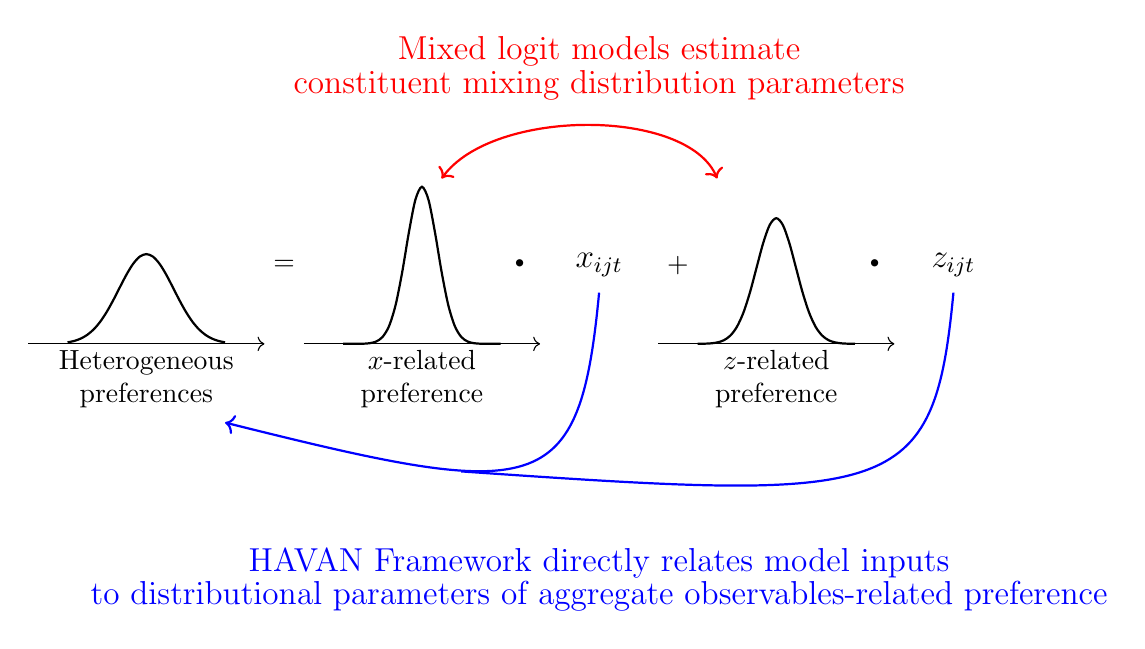
\begin{tikzpicture}
    \draw[white](0,0)--(0,0);
    \begin{scope}[shift={(0,0)}]

        \draw[->] (-1.5,0) -- (1.5,0) node[right] {};


        % Adjusted standard deviation
        \def\stddev{0.35}

        % Normal distribution curve
        \draw[smooth, thick, domain=-1:1] plot (\x, {exp(-\x*\x/(2*\stddev*\stddev))/(sqrt(2*pi)*\stddev)});



    \end{scope}



    \node[black] at (1.75,1) {=};

    \node[black] at (4.75,1) {\Huge $\cdot$};
    \node[black] at (5.75,1) {\large $x_{ijt}$};
    \node[black] at (6.75,1) {+};
    \node[black] at (9.25,1) {\Huge $\cdot$};
    \node[black] at (10.25,1) {\large $z_{ijt}$};
    \node[black, align=center] at (8,-.45) {$z$-related\\preference};
    \node[black, align=center] at (3.5,-.45) {$x$-related\\preference};

    \node[black, align=center] at (0,-.45) {Heterogeneous\\preferences};
    \begin{scope}[shift={(8,0)}]

        \draw[->] (-1.5,0) -- (1.5,0) node[right] {};


        % Adjusted standard deviation
        \def\stddev{0.25}

        % Normal distribution curve
        \draw[smooth, thick, domain=-1:1] plot (\x, {exp(-\x*\x/(2*\stddev*\stddev))/(sqrt(2*pi)*\stddev)});



    \end{scope}

    \begin{scope}[shift={(3.5,0)}]

        \draw[->] (-1.5,0) -- (1.5,0) node[right] {};


        % Adjusted standard deviation
        \def\stddev{0.2}

        % Normal distribution curve
        \draw[smooth, thick, domain=-1:1] plot (\x, {exp(-\x*\x/(2*\stddev*\stddev))/(sqrt(2*pi)*\stddev)});



    \end{scope}

    \draw[red, <->, thick] (3.75, 2.1) .. controls (4.4,3) and (6.875,3) .. (7.25, 2.1);
    \node[red, align=center] at (5.75,3.5) {\large Mixed logit models estimate\\ \large constituent mixing distribution parameters};
    \draw[blue, ->, thick] (5.75, .65) .. controls (5.5,-2) and (5,-2) .. (1, -1);
    \draw[blue, -, thick] (10.25, .65) .. controls (10,-2) and (9.5,-2) .. (4, -1.62);
    \node[blue, align=center] at (5.75,-3) {\large HAVAN Framework directly relates model inputs\\ \large to distributional parameters of aggregate observables-related preference};
\end{tikzpicture}

\end{document}